\documentclass{article}

\usepackage[preprint]{neurips_2025}

\usepackage{amsmath,amssymb}
\usepackage{booktabs}
\usepackage{graphicx}
\usepackage{hyperref}

\title{Post-Training Typed-Decision Models with Proper-Scoring Losses:\\Accuracy, Calibration, and Soft-Target Underconfidence}
\author{Sai Krishna Rallabandi}

\begin{document}
\maketitle

\begin{abstract}
Typed-decision models answer choice, score, and yes/no questions about a
state in one forward pass and report a probability distribution that
downstream thresholds consume. We post-train such models (Kev, a
prefill-only pointer-head reconstruction of TypeSafe's Jev) with
cross-entropy against soft gold distributions plus Brier and
ranked-probability-score terms, at two scales and two data regimes. On 400
held-out business-decision cases, a 4B delta raises decision accuracy from
0.665 to 0.800 and cuts KL from gold threefold (0.226 to 0.079), while ECE
regresses from 0.091 to 0.162. A cold-started 9B replication reproduces the
pattern (0.774 accuracy, ECE 0.149), and a 9B model trained on a 13.4k-record
mixture (v2) reaches 0.783. The ECE regression is \emph{underconfidence} in
every confidence bin and every question type: the expected signature of
matching soft targets and then scoring against discrete labels. A single
temperature below one, fit group-disjointly, restores ECE (4B: 0.009;
9B: 0.021) with accuracy unchanged, at a large cost in fidelity to the gold
distribution (KL 0.079 to 0.469 at 4B). The sign of miscalibration is a
property of the evaluation distribution, not of the model: the same v2
model is \emph{overconfident} (bias $+0.107$) on 6,264 external hard-label
decisions, so the in-domain temperature must not be shipped as a global
fix.
\end{abstract}

\section{Introduction}

Autonomous systems increasingly act on model outputs without a human in the
loop: routing tickets, triaging incidents, approving invoices. Each act is a
\emph{typed decision}, meaning a choice among named options, a score on an
ordered scale, or a yes/no verdict, reported as a probability distribution.
Downstream thresholds (automate, defer, escalate) are only meaningful if
0.80 means right 80\% of the time. A family of single-pass ``System One''
decision models now targets this interface: the hosted Jev, open
reconstructions such as Kev~\cite{kev2026}, Laya~\cite{laya2026} and
AnyJev~\cite{zhang2026anyjev}, and domain models such as
SearchJev~\cite{cao2026searchjev}. How to post-train them so that the
reported distribution is both accurate and calibrated is an open,
practical question.

The recipe space is now crowded. RLCR~\cite{damani2025rlcr} shows that
correctness plus a bounded proper scoring rule incentivises calibrated
verbalised confidence. SearchJev~\cite{cao2026searchjev} trains Qwen3.5
LoRA decision models on soft targets with cross-entropy plus a Brier term,
then fits a temperature per output type. Laya~\cite{laya2026} post-trains
with proper-scoring RL rewards, including RPS for ordinal questions. What
these reports do not provide is a diagnosis: in which \emph{direction} the
resulting model is miscalibrated, on which question types, how that changes
under distribution shift, and what post-hoc correction costs in fidelity to
the gold distribution. Those are the quantities a deployment needs to set
thresholds, and they are what this paper measures.

We post-train Kev models with soft-target cross-entropy plus Brier and RPS
terms and evaluate them on a fixed typed-decision benchmark with
distributional gold. Our contributions are empirical:
\begin{itemize}
\item \textbf{Proper-loss post-training improves accuracy, proper scores and
selective prediction together}, at 4B (0.665 to 0.800) and in a
cold-started 9B replication (0.774), with gains in every workflow and
question type (Section~\ref{sec:results}).
\item \textbf{The resulting miscalibration is underconfidence}, in every
bin and every primitive, worst on ordinal score questions (ECE 0.212). This
is the predicted signature of matching soft targets and then scoring
against majority labels~\cite{baan2022stop,kohli2026saturation}. The
released Kev checkpoints, trained on hard labels, ship temperatures above
two~\cite{kev2026}; our deltas from the same family need $T\approx0.4$. An
independently trained Laya specialist on the same split is
underconfident too (Section~\ref{sec:analysis}).
\item \textbf{One temperature restores ECE, with an explicit fidelity
cost and no transfer guarantee.} Group-disjoint temperatures bring ECE to
0.009 (4B) and 0.021 (9B) with accuracy fixed, but triple-to-sextuple KL
from gold. On external hard-label data, the v2 model is overconfident, so
the in-domain $T<1$ points the wrong way (Section~\ref{sec:results}).
\end{itemize}

\begin{figure}[t]
\centering
\begin{minipage}{0.92\linewidth}\small
\textbf{Running example (invoice\_processing\_000008, held out).} Invoice
INV-2026-6038 (\$36,720, Acme Fabrication) against PO-4946; delivery
accepted with exceptions, received quantity 0. Gold vs.\ 4B delta:
\texttt{discrepancy\_severity} (score): gold $\{3{:}0.83\}$ vs.\ model
$\{3{:}0.62, 2{:}0.30\}$; \texttt{disposition} (choice): gold
$\{\text{manual\_review}{:}0.57, \text{hold}{:}0.34\}$ vs.\ model
$\{\text{manual\_review}{:}0.50, \text{hold}{:}0.43\}$;
\texttt{duplicate} (noul): gold $\{\text{false}{:}0.96\}$ vs.\ model
$\{\text{false}{:}0.95\}$; \texttt{matches\_order} (noul): gold
$\{\text{false}{:}0.92\}$ vs.\ model $\{\text{false}{:}0.89\}$;
\texttt{urgency} (score): gold $\{2{:}0.50, 1{:}0.37\}$ vs.\ model
$\{2{:}0.56, 1{:}0.27\}$. All five argmax decisions are correct, and the
predicted mass tracks the gold mass with slightly wider spread.
\end{minipage}
\caption{A real held-out case: gold distributions and measured 4B-delta
outputs. Section~\ref{sec:method} uses its \texttt{urgency} question.}
\label{fig:running}
\end{figure}

\section{Background and Related Work}

\paragraph{System One decision models.} TypeSafe's Jev answers typed
questions in one pass and is post-trained with an undisclosed procedure
called RLCD~\cite{typesafe2026rlcd}. Kev~\cite{kev2026} is an open
reconstruction: a causal LM run prefill-only, LoRA adapters, and a pointer
head that scores option-boundary tokens, trained with cross-entropy on
hard-label decision suites and shipped with a built-in temperature ($T=2.41$
at 4B, $2.30$ at 9B). AnyJev~\cite{zhang2026anyjev} reads decisions from an
untrained LM in one prefill. Laya~\cite{laya2026} post-trains with
proper-scoring RL rewards (log and spherical, plus RPS for ordinal
questions). SearchJev~\cite{cao2026searchjev} is closest to our recipe: it
fits soft target distributions with cross-entropy plus $0.5\cdot$Brier on
Qwen3.5 LoRA models and fits per-output-type temperatures on 5,000
validation decisions. It reports neither the fitted temperatures nor the
direction of miscalibration. Evaluations of this family compare it with
fine-tuned encoders and generative LLMs~\cite{rafe2026benchmarking} and
report finite-sample noise floors for ECE~\cite{sharma2026typedbench};
TypedBench finds Jev itself underconfident after refitting.

\paragraph{Calibration under soft supervision.} Modern networks trained with
cross-entropy are typically overconfident and are repaired by temperature
scaling~\cite{guo2017calibration,desai2020calibration}. Softened targets
push the other way. Label smoothing and soft-label augmentation produce
underconfidence that compounds with other
regularisers~\cite{muller2019labelsmoothing,wen2021ensembles}, and models
trained with such regularisation are harder to recalibrate
post hoc~\cite{wang2021rethinking}. When the gold itself is a distribution
of human or teacher judgments, scoring calibration against the majority
label penalises a model that correctly reports the
disagreement~\cite{baan2022stop,nie2020chaosnli}. On ChaosNLI, soft-label
training lowers KL and raises majority-label ECE, exactly our
pattern~\cite{kohli2026saturation}. Temperatures fit on discrete labels are
biased towards understating annotator
uncertainty~\cite{tao2026ambiguous,dogah2026tsnotenough}. Our results
should therefore be read as a measurement of a predicted effect in a new
model family, not as the discovery of a new phenomenon.

\paragraph{RL and proper scores.} RLCR~\cite{damani2025rlcr} proves that
correctness plus a bounded proper rule (Brier, not log loss) incentivises
calibrated verbalised confidence. Follow-ups place confidence rewards on an
overconfidence--underconfidence spectrum~\cite{tan2026rewardfunctions}.
Verifiable-reward RL produces overconfident decision tokens that inherit
calibration from reasoning traces~\cite{yaldiz2026calibration}. Our models
have no reasoning trace and report the decision distribution itself as
confidence. After temperature scaling, proper-score objectives are not
clearly better calibrated than cross-entropy~\cite{deka2026sbert2s1}, which
matches our finding that post-hoc temperature, not the loss, is what
sets ECE.

\section{Method}
\label{sec:method}

A case is a state $s$ (JSON) and questions $q$, each with $k_q$ options and
a soft gold distribution $g$ obtained by averaging teacher judgments; $y$ is
its argmax. The model is a Kev pointer head: logits $z \in \mathbb{R}^{k_q}$
at option-boundary tokens of a prefill-only causal LM, $p =
\mathrm{softmax}(z)$. Training minimises, per decision,
\[
\mathcal{L} = \mathrm{CE}(p, g) + 0.5\cdot\mathrm{Brier}(p, y)
+ 0.5\cdot\mathrm{RPS}(p, y),
\]
with the RPS term~\cite{epstein1969rps} only on score questions. Both
auxiliary terms are strictly proper~\cite{gneiting2007proper} and are
scored against the realised label $y$, whereas SearchJev's Brier term is
scored against $g$. Adaptation is LoRA (rank 16, $\alpha=32$, all
projections) plus the pointer head.

For \texttt{urgency} in Figure~\ref{fig:running} (gold
$\{2{:}0.50, 1{:}0.37, 3{:}0.10, 0{:}0.03\}$), a hard-label trainer pushes
all mass to level~2. The soft cross-entropy term instead penalises starving
level~1 of its 0.37, and the measured output $\{2{:}0.56, 1{:}0.27,
3{:}0.14, 0{:}0.03\}$ tracks the gold spread. That spread is what the loss
asks for, and it is also why argmax confidence (0.56) understates argmax
accuracy on the test set.

\paragraph{Temperature.} Inference reports $\mathrm{softmax}(z/T)$, which
leaves the argmax unchanged. We report two fits, both minimising NLL against
$y$. (i)~\emph{Train-fit}: $T$ on the model's own training split, on a 0.05
grid (4B only; $T^\star=0.35$). The model has seen these rows, so this fit
is in-distribution by construction. (ii)~\emph{Cross-fit}: five-fold
group-disjoint fits on the test set, where each fold's $T$ comes from the
other four folds and all questions of a case stay in one fold (Kev's
\texttt{out\_of\_fold\_rows}, 121-point log grid on $[0.25, 4]$). Cross-fit
is the honest estimate of what a held-out calibration set from the same
distribution would give.

\section{Experimental Setup}

\paragraph{Data.} \emph{v1}: four business-decision workflows (agent-trace
observability, customer service, invoice processing, security incidents);
1,200 training cases (6,000 decisions) and 400 held-out test cases (2,000
decisions, 1,945 scored after context rejects; 778 score, 578 choice, 589
noul). Gold distributions average teacher judgments (mean entropy
0.75 nats). Rare labels have fewer than 15 training occurrences
(e.g.\ \texttt{action=stop}), which bounds tail-calibration claims.
\emph{v2}: 13,423 training records adding HelpSteer2 (score),
UltraFeedback-binarised, MMLU auxiliary-train, HellaSwag and ANLI-R1
(choice), grouped-soft hate-speech ratings (score) and PubMedQA (noul) to
v1. The v2 evaluation set has 6,264 scored decisions: a 12\% per-source
hold-out plus ChaosNLI~\cite{nie2020chaosnli} and RewardBench, kept
evaluation-only (5,558 choice, 600 score, 106 noul). A normalised
exact-match audit against the v1 test found no leaks.

\paragraph{Models.} \emph{4B delta}: warm start from the released
kev-4b, two epochs on v1. \emph{9B delta}: cold start from
Qwen3.5-9B-Base (no trusted 9B adapter to warm-start from), same recipe.
\emph{v2-9B}: warm start from the 9B delta, two epochs on v2. Shared
hyperparameters: lr $2\times10^{-5}$, batch $1\times8$ accumulation,
gradient checkpointing, no option permutation, seed 0, one fixed
configuration with no search. Compute: one RTX 3090 for v1 (about 2~h at 4B
and 75~min at 9B), one A6000 for v2 (about 20~h).

\paragraph{Baselines.} The eight released and trained Kev checkpoints
(0.5B to 9B) evaluated by the same harness, each at the temperature it
ships with. The Laya typed-decisions specialist, a Laya checkpoint specialised to the
same v1 training split (the Laya family is post-trained with
proper-scoring RL rewards~\cite{laya2026}). A zero-shot DeBERTa-v3 NLI
model. The specialist and NLI predictions come from our
\texttt{decisionbench} harness on all 2,000 decisions, and every other
number from \texttt{kev.benchmark} on 1,945. Train-frequency prior
accuracy is 0.484.

\paragraph{Metrics.} Decision accuracy; top-label ECE (10 equal-width
bins); confidence bias (mean confidence minus accuracy; negative means
underconfident); Brier; NLL; KL(gold$\|$pred); AURC; coverage and accuracy
at confidence $\ge0.9$; score MAE and RPS. Confidence intervals come from a
case-level bootstrap (2,000 resamples), paired where two models are
compared. Every model is a \emph{single training run}, so seed variance is
unmeasured.

\section{Results}
\label{sec:results}

\paragraph{Proper-loss post-training improves accuracy, proper scores and
selective prediction (Table~\ref{tab:main}).} At 4B, accuracy rises from
0.665 to 0.800 (paired $+0.135$, 95\% CI $[0.113, 0.157]$), Brier from
0.467 to 0.327, NLL from 0.819 to 0.576 and AURC from 0.195 to 0.071; KL
from gold falls from 0.226 to 0.079. Coverage at confidence $\ge0.9$ doubles
(0.059 to 0.130) with no errors inside the band. Gains hold in every
workflow (agent-trace 0.568 to 0.754, customer service 0.706 to 0.822,
invoice 0.692 to 0.840, security 0.700 to 0.786) and every primitive. The
cold-started 9B delta reproduces every direction (0.774 accuracy, KL 0.093)
and beats the released kev-9b by $+0.057$ $[0.035, 0.078]$. It trails the
warm-started 4B by $0.026$ $[0.010, 0.042]$. That gap is resolvable on these
items, but it confounds scale with warm-start and has no seed replicate, so
we read it as ``no gain from scale under cold start'', not as evidence
against scale.

\begin{table}[t]
\centering\small
\resizebox{\linewidth}{!}{%
\begin{tabular}{lcccccc}
\toprule
 & kev-4b & 4B delta & 4B + $T$ & 9B delta & 9B + $T$ & v2-9B \\
\midrule
decision accuracy & 0.665 & 0.800 & 0.800 & 0.774 & 0.774 & 0.783 \\
ECE & 0.091 & 0.162 & \textbf{0.009} & 0.149 & 0.021 & 0.140 \\
confidence bias & $-0.089$ & $-0.162$ & $+0.005$ & $-0.149$ & $+0.007$ & $-0.140$ \\
Brier & 0.467 & 0.327 & \textbf{0.276} & 0.350 & 0.310 & 0.334 \\
NLL & 0.819 & 0.576 & \textbf{0.460} & 0.612 & 0.511 & 0.585 \\
KL(gold$\|$pred) & 0.226 & \textbf{0.079} & 0.469$^\dagger$ & 0.093 & 0.302 & --- \\
AURC & 0.195 & 0.071 & \textbf{0.069} & 0.087 & 0.085 & 0.079 \\
coverage / acc.\ at conf.\ $\ge$0.9 & .059 / .983 & .130 / 1.00 & .374 / .974 & .120 / 1.00 & .319 / .977 & .133 / 1.00 \\
score ECE & 0.074 & 0.212 & 0.034 & 0.198 & 0.044 & 0.196 \\
choice / noul ECE & .104 / .111 & .149 / .107 & .051 / .012 & .131 / .104 & .056 / .022 & .135 / .084 \\
\bottomrule
\end{tabular}}
\caption{Held-out v1 test (400 cases, 1,945 decisions). ``$+T$'' is the
five-fold group-disjoint cross-fit temperature ($T\approx0.41$ at 4B, $0.45$
at 9B). ECE 95\% CIs: 4B $[0.143, 0.180]$ raw, $[0.009, 0.030]$ cross-fit;
9B $[0.131, 0.168]$, $[0.013, 0.039]$. $^\dagger$KL at the train-fit
$T^\star=0.35$ (ECE 0.032, NLL 0.464). v2-9B logits were not retained, so
its temperature-scaled and KL columns are not computed. kev-4b is scored at
its shipped $T=2.41$.}
\label{tab:main}
\end{table}

\paragraph{ECE regresses because the deltas are underconfident.} Raw ECE
rises from 0.091 to 0.162 at 4B and sits at 0.149 at 9B, with confidence
bias equal to $-$ECE. In other words, the model is underconfident in
aggregate, and Figure~\ref{fig:scale} shows it is underconfident in every
bin at both scales. Score questions carry most of it (0.212 and 0.198);
noul is mildest. More data does not remove it: v2-9B is still at $-0.140$
on the v1 test.

\paragraph{A temperature below one restores ECE, and the cost is KL.}
Cross-fit temperatures are stable across folds (4B: 0.40--0.43; 9B:
0.44--0.46) and bring ECE to 0.009 and 0.021, with Brier and NLL improving
and accuracy fixed. Selective prediction becomes usable: at confidence
$\ge0.9$ the 4B model now covers 37.4\% of decisions at 97.4\% accuracy,
against 13.0\% before. The train-fit $T^\star=0.35$ at 4B gives 0.032, which
is consistent. Per-primitive temperatures are similar to the global one at
9B (choice 0.52, noul 0.44, score 0.40; ECE 0.045, 0.007, 0.017), so one
global $T$ suffices in-domain. Sharpening, however, moves the output away
from the gold distributions it was trained to match: KL rises from 0.079
to 0.469 at 4B and from 0.093 to 0.302 at 9B. A deployment has to choose
between probabilities that match annotator disagreement and probabilities
that match argmax hit rates. One temperature cannot give both.

\paragraph{Under shift, the sign flips.} On the 6,264-decision v2
evaluation set, which is dominated by external sources with near-hard
labels, v2-9B reaches 0.786 accuracy (choice 0.801, score 0.647, noul
0.783), but it is \emph{overconfident}: mean confidence 0.893, bias
$+0.107$ (choice $+0.114$, noul $+0.145$, score $+0.035$). At confidence
$\ge0.9$ it covers 69\% of decisions at 87.2\% accuracy, against 100\% on
the v1 test. Any $T<1$ fit in-domain would raise these confidences further.
The direction of miscalibration is a property of how soft the evaluation
labels are relative to the training targets, not a fixed property of the
model.

\paragraph{Fair comparison with the baselines (Table~\ref{tab:sweep}).}
The Laya typed-decisions specialist is also underconfident on this data
(bias $-0.214$). With the same cross-fit, its ECE falls from 0.214 to 0.018
($T\approx0.33$). After temperature scaling, our 4B delta and the
specialist are therefore comparably calibrated (0.009 vs.\ 0.018), and our
advantage is accuracy (0.800 vs.\ 0.767) and Brier (0.276 vs.\ 0.318).
The NLI baseline is mildly overconfident ($T\approx1.46$), and temperature
does not improve its ECE (0.081 to 0.089). Among the released Kev models,
accuracy grows with size except kev-8b (Qwen3 backbone; 0.638 < kev-4b's
0.665), and the sub-1B models cluster near 0.45.

\begin{table}[t]
\centering\small
\resizebox{\linewidth}{!}{%
\begin{tabular}{lccccc}
\toprule
model & acc. & ECE & bias & Brier & ECE after cross-fit $T$ \\
\midrule
kev-0.5b / 0.6b & .455 / .447 & .114 / .227 & $+.114$ / $+.227$ & .680 / .727 & --- \\
kev-0.8b (shipped $T$=2.35) & 0.458 & 0.047 & $+0.014$ & 0.608 & --- \\
kev-8b (Qwen3) & 0.638 & 0.112 & $+0.112$ & 0.513 & 0.051 ($T\approx1.7$) \\
kev-4b (shipped $T$=2.41) & 0.665 & 0.091 & $-0.089$ & 0.467 & --- \\
kev-9b (shipped $T$=2.30) & 0.718 & 0.091 & $-0.091$ & 0.414 & --- \\
NLI zero-shot$^*$ & 0.531 & 0.081 & $+0.035$ & 0.590 & 0.089 ($T\approx1.46$) \\
Laya typed-decisions$^*$ & 0.767 & 0.214 & $-0.214$ & 0.400 & 0.018 ($T\approx0.33$) \\
4B delta (ours) & \textbf{0.800} & 0.162 & $-0.162$ & 0.327 & \textbf{0.009} ($T\approx0.41$) \\
9B delta (ours) & 0.774 & 0.149 & $-0.149$ & 0.350 & 0.021 ($T\approx0.45$) \\
\bottomrule
\end{tabular}}
\caption{All models on the v1 test. $^*$\texttt{decisionbench} harness,
2,000 decisions; all others \texttt{kev.benchmark}, 1,945--1,955. Models
that ship a temperature are not refit, because their recorded logits
already include it. Hard-label-trained Kev models without a shipped
temperature are overconfident ($+$); every soft-target-trained model is
underconfident.}
\label{tab:sweep}
\end{table}

\section{Analysis and Limitations}
\label{sec:analysis}

\begin{figure}[t]
\centering
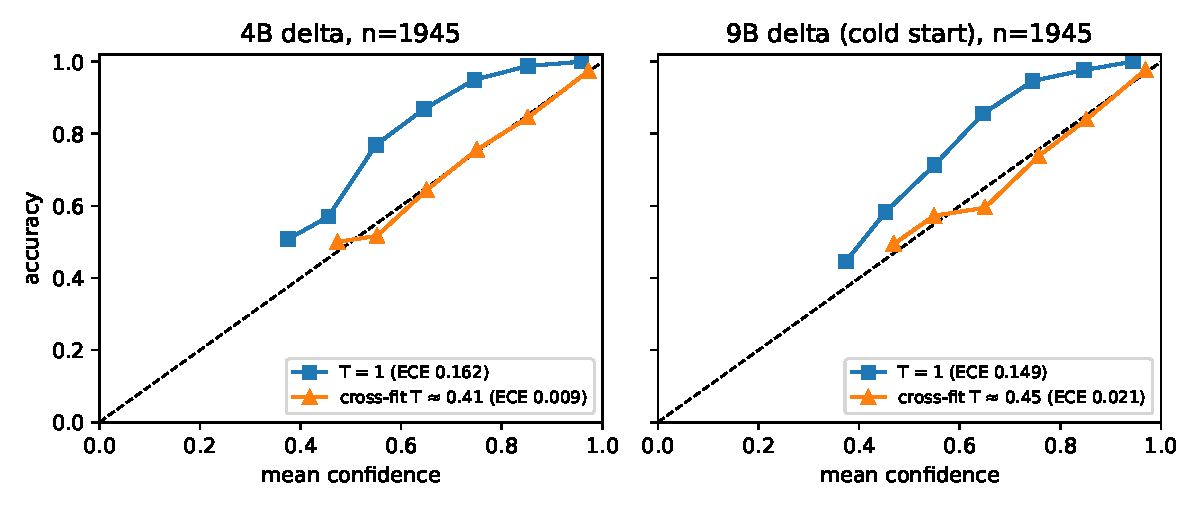
\includegraphics[width=0.92\linewidth]{fig_reliability_scale.pdf}
\caption{Reliability on the v1 test (accuracy vs.\ mean confidence, 10
bins, bins with $\ge10$ decisions). At $T=1$ both deltas lie \emph{above}
the diagonal, meaning they are underconfident in every bin. The cross-fit
temperature brings both onto it.}
\label{fig:scale}
\end{figure}

\paragraph{Mechanism.} The cross-entropy term is minimised when $p=g$, and
the gold here has 0.75 nats of mean entropy, so the trained model reports
spread-out distributions. The argmax of those distributions is right more
often than its probability says, because the teacher's majority label is
usually the gold argmax. ECE scored against $y$ therefore reads
underconfidence~\cite{baan2022stop,kohli2026saturation}. Two observations
outside our own runs support this. The released Kev models, trained with
hard-label cross-entropy, are overconfident before their shipped
temperatures ($T>2$), while our deltas from the same family need $T<1$.
And the independently trained Laya specialist on the same split is
underconfident with a similar fitted temperature (0.33 vs.\ 0.41). This is not a
controlled hard-versus-soft comparison: data, starting point and training
stage all differ. Running that comparison on one backbone is the obvious
next experiment.

\paragraph{What the temperature is fitting.} Both of our fits minimise NLL
against discrete labels, which is the estimator shown to understate
annotator uncertainty~\cite{tao2026ambiguous,dogah2026tsnotenough}. That is
the right target if downstream thresholds act on argmax hit rates, and the
wrong one if consumers read the probabilities as disagreement. The KL
column of Table~\ref{tab:main} quantifies that choice. Calibrators fit to
the soft gold itself are the natural comparison and are untested here.

\paragraph{Limitations.} (i)~Every model is a single training run. Seed
variance is unmeasured, and the 4B--9B gap confounds scale with
warm-start. (ii)~The train-fit temperature uses rows the model was trained
on. Cross-fit temperatures on the test distribution are honest about
held-out data from the \emph{same} distribution, but they say nothing
about shift, and the v2 evaluation shows that shift can reverse the sign.
(iii)~Tail calibration is unmeasured, because rare labels have single-digit
training counts. (iv)~The v2-9B logits were not retained, so its
temperature analysis is limited to the sign of its bias. (v)~The
temperature hypothesis was formed by inspecting test-set reliability
before the honest fits were run. We report the direction as post hoc and
the validation as not. (vi)~With 1,945 decisions, ECE values near 0.01 are
close to the finite-sample noise floor~\cite{sharma2026typedbench}, so
0.009 and 0.021 should not be ranked against each other.

\section{Conclusion}

Post-training a single-pass decision model with soft-target cross-entropy
plus Brier and RPS terms improves accuracy, proper scores and selective
prediction at 4B and 9B. It also makes the model underconfident against
discrete labels, as the soft-label calibration literature predicts. One
temperature below one repairs in-domain ECE without touching accuracy, but
it trades away the distributional fidelity the loss bought, and it points
the wrong way on external hard-label data, where the same model is
overconfident. The practical rule is to fit temperatures per deployment
distribution, against the label semantics the thresholds will use, and
never ship a training-distribution temperature as a global constant.

\bibliographystyle{plain}
\bibliography{references}

\end{document}
